\documentclass[12pt]{article}
\usepackage[utf8]{inputenc}
\usepackage[spanish]{babel}
\usepackage{geometry}
\geometry{a4paper, margin=1in}
\usepackage{amsmath} % Para ecuaciones (aunque no haya explícitamente, es estándar en docs técnicos)
\usepackage{graphicx} % Para incluir imágenes
\usepackage{hyperref} % Para enlaces
\usepackage{enumitem} % Para listas personalizadas si es necesario
\usepackage{fancyhdr} % Para encabezados/pies de página personalizados (opcional)
\usepackage{xcolor} % Para colores si se necesitan

% Configuración para URL más legibles
\hypersetup{
    colorlinks=true,
    linkcolor=blue,
    filecolor=magenta,
    urlcolor=cyan,
}

% --- Comandos personalizados para secciones si se quiere más control ---
% \newcommand{\seccion}[1]{\section*{#1}}
% \newcommand{\subseccion}[1]{\subsection*{#1}}
% \newcommand{\parrafo}[1]{\paragraph*{#1}}

\title{Predicción de la Cobertura de Nieve con Modelos NARX-LSTM}
\author{Enrique José Merino Arribas}
\date{}

\begin{document}

\maketitle % Genera el título

\section*{\texorpdfstring{\textsuperscript{\(\text{\char"2744}\)} Visión General del Proyecto}{Visión General del Proyecto}}
Este proyecto se enfoca en la predicción del área de nieve en seis cuencas hidrográficas específicas utilizando modelos \textbf{NARX (Nonlinear Autoregressive with Exogenous Inputs)} implementados con capas \textbf{LSTM (Long Short-Term Memory)}. El objetivo es generar predicciones futuras de la capa de nieve para apoyar la gestión hídrica y la prevención de riesgos.

\section*{\texorpdfstring{\textsuperscript{\(\text{\char"1F3AF}\)} Objetivo del Modelo}{Objetivo del Modelo}}
La finalidad de este código es utilizar modelos de redes neuronales LSTM, previamente entrenados para cada cuenca, para predecir el \texttt{area de nieve}. Las predicciones se basan en el historial del \texttt{area de nieve} extraido del satélite MODIS(componente auto-regresivo) y en variables meteorológicas externas (componente exógeno).

\section*{\texorpdfstring{\textsuperscript{\(\text{\char"1F9E0}\)} Tipo de Modelo: NARX con LSTM}{Tipo de Modelo: NARX con LSTM}}
Nuestros modelos utilizan la arquitectura \textbf{NARX} por su capacidad para predecir series temporales combinando:
\begin{itemize}
    \item \textbf{Auto-Regresión (AR):} Dependencia de valores pasados del \texttt{area\_nieve}.
    \item \textbf{Variables Exógenas (X):} Influencia de otras variables como \texttt{temperatura}, \texttt{precipitacion}, y \texttt{dias\_sin\_precip}.
    \item \textbf{No Linealidad (N):} Implementación con \textbf{capas LSTM} para capturar relaciones complejas y dependencias a largo plazo en los datos secuenciales, evitando problemas como el gradiente desvanecido de RNNs básicas.
\end{itemize}

\subsection*{Arquitectura Común del Modelo}
Cada cuenca tiene un modelo NARX-LSTM independiente. La arquitectura base es:
\begin{itemize}
    \item \textbf{Capa de Entrada:} Recibe secuencias de \texttt{n\_lags\_area} (ej. 3 días) de \texttt{area\_nieve} y variables exógenas escaladas.
    \begin{itemize}
        \item Formato: \texttt{input\_shape = (n\_lags\_area, 1 + num\_variables\_exogenas)}
    \end{itemize}
    \item \textbf{Capa LSTM:} Procesa las secuencias, aprendiendo patrones temporales.
    \begin{itemize}
        \item Configurable con \texttt{n\_units\_lstm} (número de neuronas, ej. 10, 20, 50) y activación \texttt{relu}.
    \end{itemize}
    \item \textbf{Capa Densa de Salida:} Una única neurona que produce la predicción del \texttt{area\_nieve} para el siguiente paso (\textit{t+1}).
\end{itemize}

\section*{\texorpdfstring{\textsuperscript{\(\text{\char"1F4C9}\)} Estructura de los Datos}{Estructura de los Datos}}
Los datos son obtenidos del satélite \textbf{MOD10A1F de la NASA (\href{https://search.earthdata.nasa.gov/search}{EarthData Search})} y consisten principalmente en:
\begin{itemize}
    \item \textbf{\texttt{CGF\_NDSI\_Snow\_Cover}:} (Variable de interés) Índice de Nieve de Diferencia Normalizada. Valores entre \texttt{40} y \texttt{100} indican \textbf{nieve}. Otros valores son datos nulos, nubes, agua, etc.
    \item \textbf{\texttt{Cloud\_Persistence}:} Conteo de días consecutivos con cobertura de nubes.
\end{itemize}
Ambos son datos ráster procesados para obtener el \texttt{area\_nieve} diaria por cuenca y luego combinados con series temporales de variables meteorológicas.

\subsection*{Procesamiento Inicial de Datos}
\begin{enumerate}
    \item \textbf{Obtención:} Datos MODIS descargados de \href{https://search.earthdata.nasa.gov/search}{EarthData Search}, filtrados por fecha y área (\texttt{.shp} de cuenca), reproyectados a latitud/longitud.
    \item \textbf{Limpieza:} Lectura de archivos \texttt{.hdf}, cálculo de \texttt{area\_nieve} diaria, lectura de series históricas de temperatura y precipitación.
    \item \textbf{Preparación:} Normalización y limpieza de series agregadas, separación en CSVs individuales por cuenca.
    \item \textbf{Ingeniería de Características:} Adición de la columna \texttt{dias\_sin\_precip} para registrar el tiempo desde la última lluvia/nieve.
\end{enumerate}

\section*{\texorpdfstring{\textsuperscript{\(\text{\char"1F680}\)} Esquema de Predicción Iterativa}{Esquema de Predicción Iterativa}}
El modelo predice el \texttt{area\_nieve} un día a la vez, utilizando sus propias predicciones anteriores como entrada para los pasos futuros (excepto las variables exógenas, que son datos reales).

Para predecir el \texttt{area\_nieve} en el día \textit{t+1}, el modelo utiliza:
\begin{itemize}
    \item Las predicciones de \texttt{area\_nieve} de los días \textit{t, t-1, ..., t - n\_lags\_area}.
    \item Los valores reales de las variables exógenas para el día \textit{t+1}.
\end{itemize}
Este proceso se repite para cada día futuro, propagando las predicciones del \texttt{area\_nieve}.

\section*{\texorpdfstring{\textsuperscript{\(\text{\char"1F9EA}\)} Tratamiento de Outliers y Mejora de Métricas}{Tratamiento de Outliers y Mejora de Métricas}}
Se identificaron \textbf{outliers significativos} en la variable \texttt{area de nieve} para las cuencas \textbf{Indrawati-Melamchi} y \textbf{Genil-Dilar}.
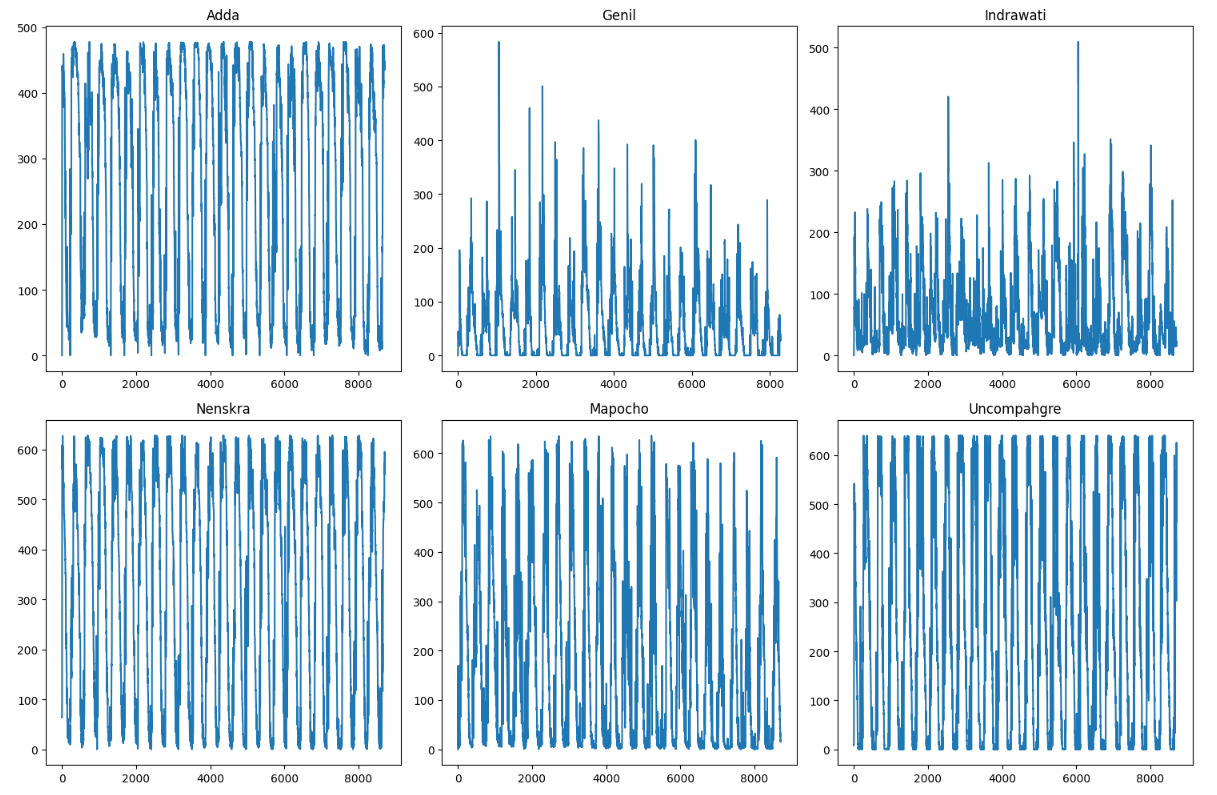
\includegraphics{lineplots_cuencas}

Para mitigar su impacto en el entrenamiento del modelo y mejorar la estabilidad de las predicciones, se han imputado estos outlayers mediante la funcion \textit{impute_outliers}:
Se han considerado outliers los valores por encima de 1.5 * \textit{rango_intercuartílico}.
Se imputarán las vairables de 'area_nieve, 'temperatura' y 'precipitacion' de las 6 cuencas y se guardarán estos datasets imputados en el directorio \textit{dataset_imputed} con lo cual se procederá a crear y evaluar distintos modelos para estos nuevos dataset y se compararán con los datasets originales para ver si se obtienen mejores métricas.

\section*{\texorpdfstring{\textsuperscript{\(\text{\char"1F4CA}\)} Métricas de Rendimiento por Modelo (Archivos \texttt{.h5})}{Métricas de Rendimiento por Modelo (Archivos .h5)}}
Cada modelo entrenado está guardado en un archivo \texttt{.h5} y su rendimiento se evalúa con las siguientes métricas en diferentes conjuntos de datos:
\begin{itemize}
    \item \textbf{R2 (Coeficiente de Determinación):} Proporción de la varianza explicada.
    \item \textbf{MAE (Error Absoluto Medio):} Error promedio en las mismas unidades que el \texttt{area\_nieve}.
    \item \textbf{NSE (Eficiencia de Nash-Sutcliffe):} Métrica hidrológica (1.0 = ajuste perfecto).
    \item \textbf{KGE (Eficiencia de Kling-Gupta):} Métrica hidrológica mejorada (1.0 = óptimo).
\end{itemize}

Las métricas se presentan para:
\begin{enumerate}
    \item \textbf{Entrenamiento:} Rendimiento sobre los datos usados para entrenar.
    \item \textbf{Prueba (Directa):} Generalización sobre datos no vistos, prediciendo un paso adelante.
    \item \textbf{Validación (Iterativa/Paso a Paso):} Robustez del modelo en predicciones a futuro, usando sus propias salidas como entradas.
    \item \textbf{Todo el Conjunto (Predictivo):} Visión global del rendimiento en modo predicción.
\end{enumerate}

A continuación, se detallan las métricas para cada modelo:

\subsection*{Adda-Bormio (\texttt{modelo\_adda\_bormio.h5})}
\begin{itemize}
    \item \textbf{Prueba (Directa):}
    \begin{itemize}
        \item R2: [Valor\_R2\_Adda\_Prueba]
        \item MAE: [Valor\_MAE\_Adda\_Prueba]
        \item NSE: [Valor\_NSE\_Adda\_Prueba]
        \item KGE: [Valor\_KGE\_Adda\_Prueba]
    \end{itemize}
    \item \textbf{Validación (Iterativa):}
    \begin{itemize}
        \item R2: [Valor\_R2\_Adda\_Val]
        \item MAE: [Valor\_MAE\_Adda\_Val]
        \item NSE: [Valor\_NSE\_Adda\_Val]
        \item KGE: [Valor\_KGE\_Adda\_Val]
    \end{itemize}
    \item \textbf{Todo el Conjunto (Predictivo):}
    \begin{itemize}
        \item R2: [Valor\_R2\_Adda\_Total]
        \item MAE: [Valor\_MAE\_Adda\_Total]
        \item NSE: [Valor\_NSE\_Adda\_Total]
        \item KGE: [Valor\_KGE\_Adda\_Total]
    \end{itemize}
\end{itemize}

\subsection*{Genil-Dilar (\texttt{modelo\_genil\_dilar.h5})}
\begin{itemize}
    \item \textbf{Prueba (Directa):}
    \begin{itemize}
        \item R2: [Valor\_R2\_Genil\_Prueba]
        \item MAE: [Valor\_MAE\_Genil\_Prueba]
        \item NSE: [Valor\_NSE\_Genil\_Prueba]
        \item KGE: [Valor\_KGE\_Genil\_Prueba]
    \end{itemize}
    \item \textbf{Validación (Iterativa):}
    \begin{itemize}
        \item R2: [Valor\_R2\_Genil\_Val]
        \item MAE: [Valor\_MAE\_Genil\_Val]
        \item NSE: [Valor\_NSE\_Genil\_Val]
        \item KGE: [Valor\_KGE\_Genil\_Val]
    \end{itemize}
    \item \textbf{Todo el Conjunto (Predictivo):}
    \begin{itemize}
        \item R2: [Valor\_R2\_Genil\_Total]
        \item MAE: [Valor\_MAE\_Genil\_Total]
        \item NSE: [Valor\_NSE\_Genil\_Total]
        \item KGE: [Valor\_KGE\_Genil\_Total]
    \end{itemize}
\end{itemize}

\subsection*{Indrawati-Melamchi (\texttt{modelo\_indrawati\_melamchi.h5})}
\begin{itemize}
    \item \textbf{Prueba (Directa):}
    \begin{itemize}
        \item R2: [Valor\_R2\_Indrawati\_Prueba]
        \item MAE: [Valor\_MAE\_Indrawati\_Prueba]
        \item NSE: [Valor\_NSE\_Indrawati\_Prueba]
        \item KGE: [Valor\_KGE\_Indrawati\_Prueba]
    \end{itemize}
    \item \textbf{Validación (Iterativa):}
    \begin{itemize}
        \item R2: [Valor\_R2\_Indrawati\_Val]
        \item MAE: [Valor\_MAE\_Indrawati\_Val]
        \item NSE: [Valor\_NSE\_Indrawati\_Val]
        \item KGE: [Valor\_KGE\_Indrawati\_Val]
    \end{itemize}
    \item \textbf{Todo el Conjunto (Predictivo):}
    \begin{itemize}
        \item R2: [Valor\_R2\_Indrawati\_Total]
        \item MAE: [Valor\_MAE\_Indrawati\_Total]
        \item NSE: [Valor\_NSE\_Indrawati\_Total]
        \item KGE: [Valor\_KGE\_Indrawati\_Total]
    \end{itemize}
\end{itemize}

\subsection*{Mapocho-Almendros (\texttt{modelo\_mapocho\_almendros.h5})}
\begin{itemize}
    \item \textbf{Prueba (Directa):}
    \begin{itemize}
        \item R2: [Valor\_R2\_Mapocho\_Prueba]
        \item MAE: [Valor\_MAE\_Mapocho\_Prueba]
        \item NSE: [Valor\_NSE\_Mapocho\_Prueba]
        \item KGE: [Valor\_KGE\_Mapocho\_Prueba]
    \end{itemize}
    \item \textbf{Validación (Iterativa):}
    \begin{itemize}
        \item R2: [Valor\_R2\_Mapocho\_Val]
        \item MAE: [Valor\_MAE\_Mapocho\_Val]
        \item NSE: [Valor\_NSE\_Mapocho\_Val]
        \item KGE: [Valor\_KGE\_Mapocho\_Val]
    \end{itemize}
    \item \textbf{Todo el Conjunto (Predictivo):}
    \begin{itemize}
        \item R2: [Valor\_R2\_Mapocho\_Total]
        \item MAE: [Valor\_MAE\_Mapocho\_Total]
        \item NSE: [Valor\_NSE\_Mapocho\_Total]
        \item KGE: [Valor\_KGE\_Mapocho\_Total]
    \end{itemize}
\end{itemize}

\subsection*{Nenskra-Enguri (\texttt{modelo\_nenskra\_enguri.h5})}
\begin{itemize}
    \item \textbf{Prueba (Directa):}
    \begin{itemize}
        \item R2: [Valor\_R2\_Nenskra\_Prueba]
        \item MAE: [Valor\_MAE\_Nenskra\_Prueba]
        \item NSE: [Valor\_NSE\_Nenskra\_Prueba]
        \item KGE: [Valor\_KGE\_Nenskra\_Prueba]
    \end{itemize}
    \item \textbf{Validación (Iterativa):}
    \begin{itemize}
        \item R2: [Valor\_R2\_Nenskra\_Val]
        \item MAE: [Valor\_MAE\_Nenskra\_Val]
        \item NSE: [Valor\_NSE\_Nenskra\_Val]
        \item KGE: [Valor\_KGE\_Nenskra\_Val]
    \end{itemize}
    \item \textbf{Todo el Conjunto (Predictivo):}
    \begin{itemize}
        \item R2: [Valor\_R2\_Nenskra\_Total]
        \item MAE: [Valor\_MAE\_Nenskra\_Total]
        \item NSE: [Valor\_NSE\_Nenskra\_Total]
        \item KGE: [Valor\_KGE\_Nenskra\_Total]
    \end{itemize}
\end{itemize}

\subsection*{Uncompahgre-Ridgway (\texttt{modelo\_uncompahgre\_ridgway.h5})}
\begin{itemize}
    \item \textbf{Prueba (Directa):}
    \begin{itemize}
        \item R2: [Valor\_R2\_Uncompahgre\_Prueba]
        \item MAE: [Valor\_MAE\_Uncompahgre\_Prueba]
        \item NSE: [Valor\_NSE\_Uncompahgre\_Prueba]
        \item KGE: [Valor\_KGE\_Uncompahgre\_Prueba]
    \end{itemize}
    \item \textbf{Validación (Iterativa):}
    \begin{itemize}
        \item R2: [Valor\_R2\_Uncompahgre\_Val]
        \item MAE: [Valor\_MAE\_Uncompahgre\_Val]
        \item NSE: [Valor\_NSE\_Uncompahgre\_Val]
        \item KGE: [Valor\_KGE\_Uncompahgre\_Val]
    \end{itemize}
    \item \textbf{Todo el Conjunto (Predictivo):}
    \begin{itemize}
        \item R2: [Valor\_R2\_Uncompahgre\_Total]
        \item MAE: [Valor\_MAE\_Uncompahgre\_Total]
        \item NSE: [Valor\_NSE\_Uncompahgre\_Total]
        \item KGE: [Valor\_KGE\_Uncompahgre\_Total]
    \end{itemize}
\end{itemize}

\end{document}